\documentclass[tikz, margin=1mm]{standalone}
\usetikzlibrary{calc}

% here a depletion thickness of 250 nanometers is shown
% the carrier density, assuming a grid, is 9/(50 nm)^3 = 7.2 e16 cm^{-3}
\begin{document}
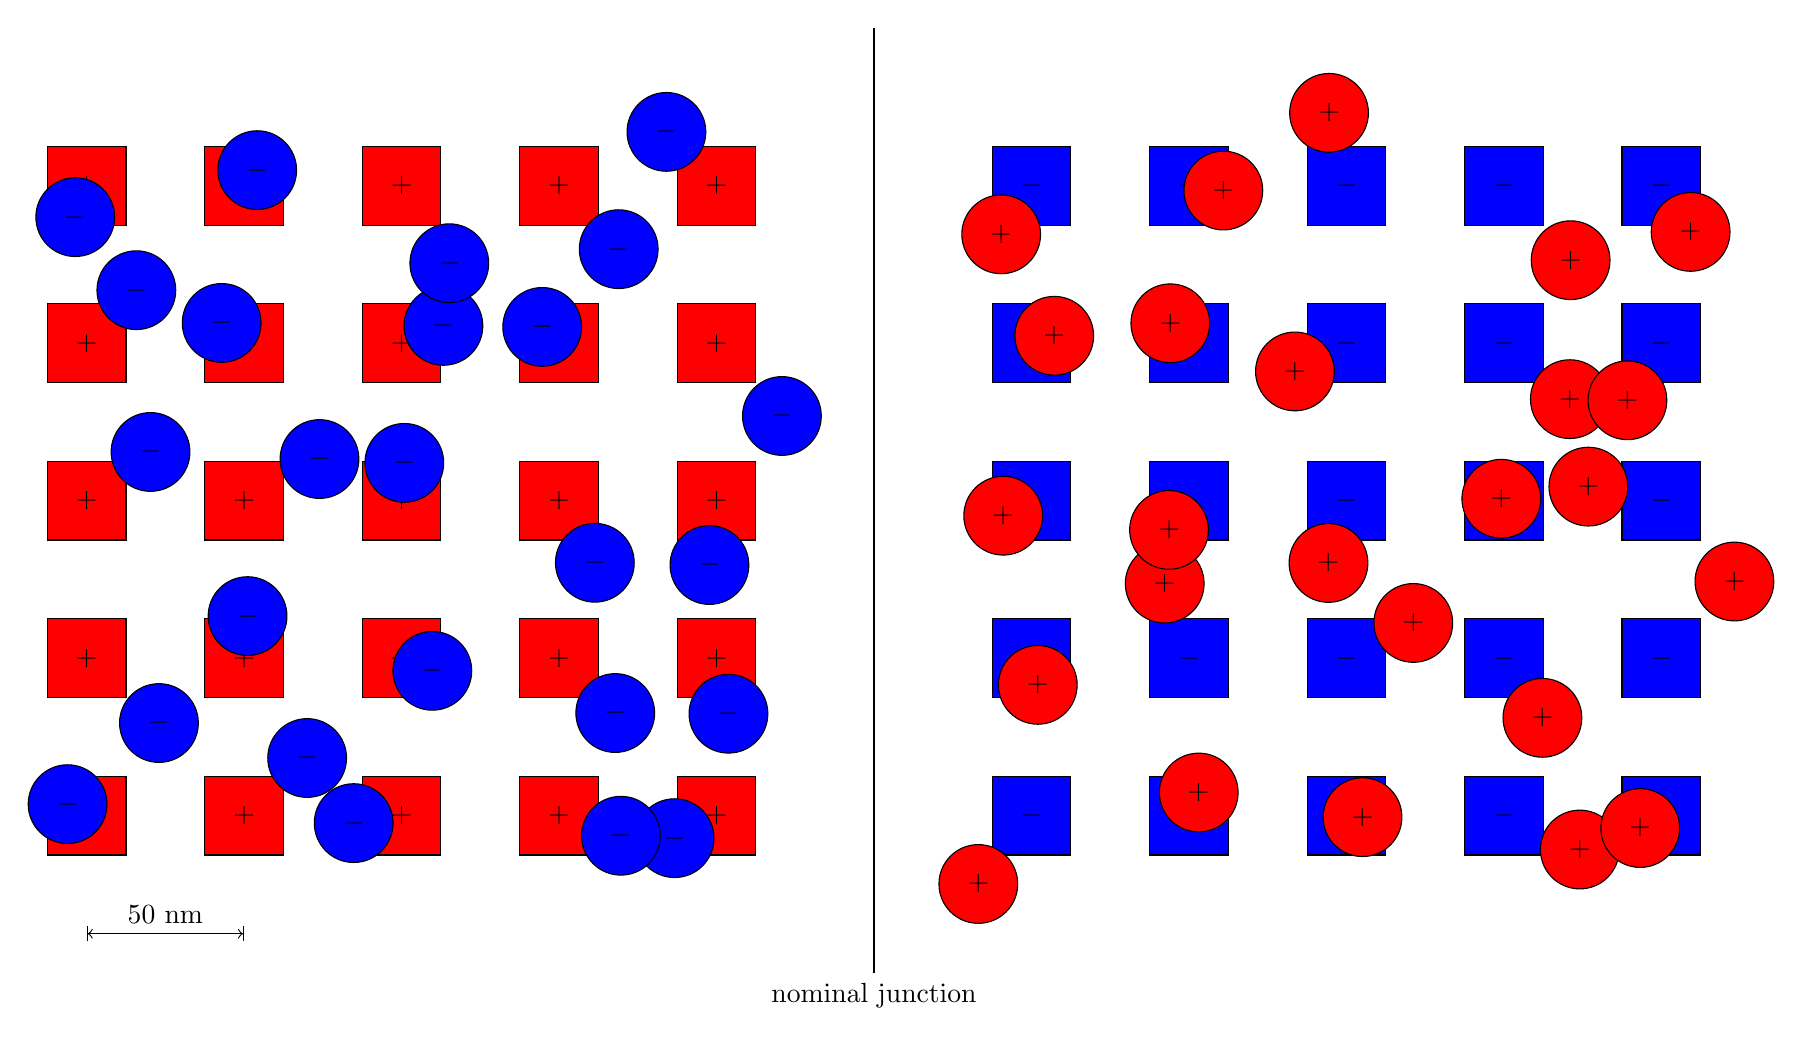
\begin{tikzpicture}
% determine canvas width

\foreach\x in {-1, -2, -3, -4, -5}
  \foreach\y in {1,2,...,5}
    {
    \node[draw, minimum size=1cm, fill=red] at ($(2*\x,2*\y)$) {$+$};
    }
\foreach\x in {-1, -2, -3, -4, -5}
  \foreach\y in {1,2,...,5}
    {
    \node[circle, draw, minimum size=1cm, fill=blue] at ($(2*\x,2*\y) + (1*rand,1*rand)$) {$-$};
    }
\foreach\x in {1, 2, 3, 4, 5}
  \foreach\y in {1,2,...,5}
    {
    \node[draw, minimum size=1cm, fill=blue] at ($(2*\x,2*\y)$) {$-$};
    }
\foreach\x in {1, 2, 3, 4, 5}
  \foreach\y in {1,2,...,5}
    {
    \node[circle, draw, minimum size=1cm, fill=red] at ($(2*\x,2*\y) + (1*rand,1*rand)$) {$+$};
    }

\draw (0, 0) -- (0, 12) node[pos=0, below] {nominal junction};
\draw[|<->|] (-10, 0.5) -- (-8,0.5) node[pos=0.5, above] {50 nm};

\end{tikzpicture}
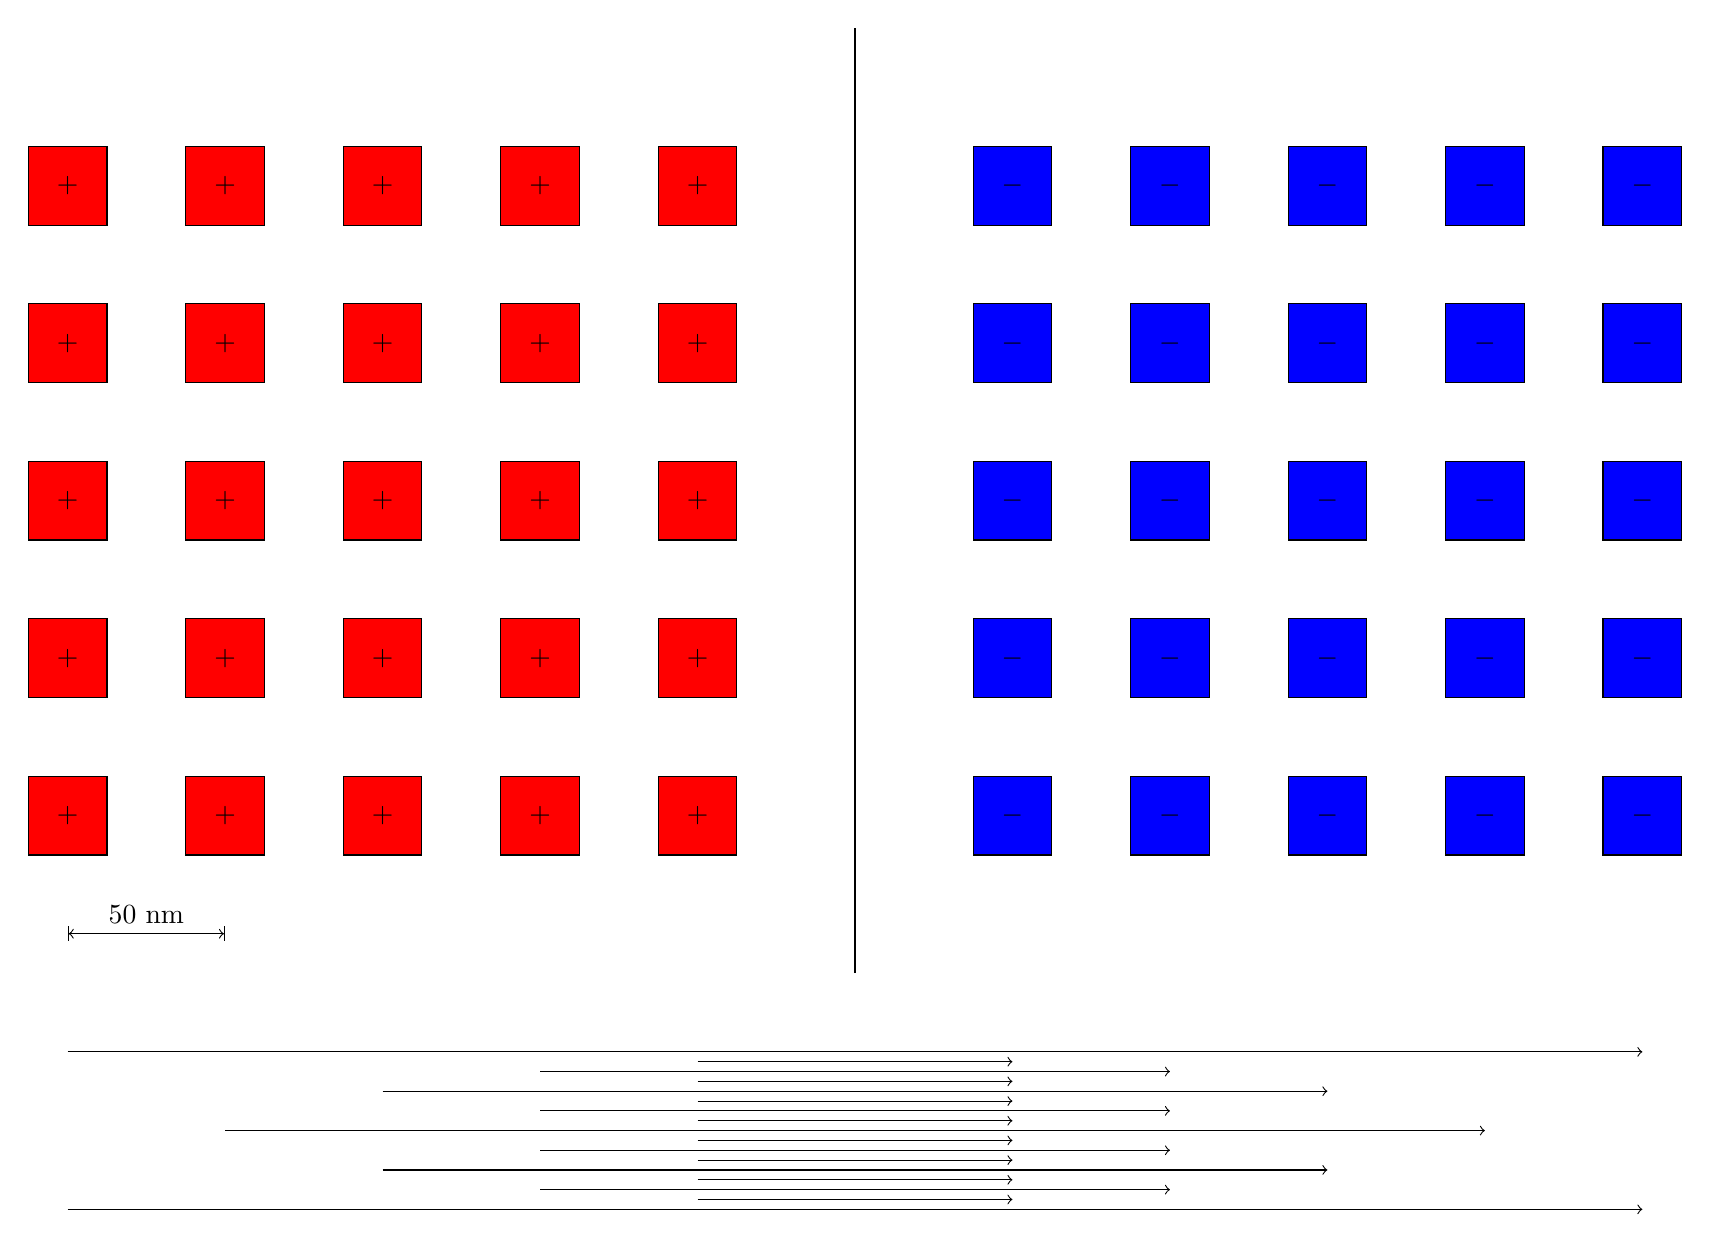
\begin{tikzpicture}

\foreach\x in {-1, -2, -3, -4, -5}
  \foreach\y in {1,2,...,5}
    {
    \node[draw, minimum size=1cm, fill=red] at ($(2*\x,2*\y)$) {$+$};
    }
\foreach\x in {1, 2, 3, 4, 5}
  \foreach\y in {1,2,...,5}
    {
    \node[draw, minimum size=1cm, fill=blue] at ($(2*\x,2*\y)$) {$-$};
    }

\draw (0, 0) -- (0, 12);
\draw[|<->|] (-10, 0.5) -- (-8,0.5) node[pos=0.5, above] {50 nm};

\draw[->] (-10, -1) -- (10, -1); %\foreach\x in {-5,-4,-3,-2,-1,0}
\draw[->] (-10, -3) -- (10, -3);
% first bisection
\draw[->] (-8, -2) -- (8, -2);
% second bisection
\draw[->] (-6, -2.5) -- (6, -2.5);
\draw[->] (-6, -1.5) -- (6, -1.5);
% third bisection
\draw[->] (-4, -2.25) -- (4, -2.25);
\draw[->] (-4, -2.75) -- (4, -2.75);
\draw[->] (-4, -1.75) -- (4, -1.75);
\draw[->] (-4, -1.25) -- (4, -1.25);
% fourth bisection
\draw[->] (-2, -2.875) -- (2, -2.875);
\draw[->] (-2, -2.625) -- (2, -2.625);
\draw[->] (-2, -2.375) -- (2, -2.375);
\draw[->] (-2, -2.125) -- (2, -2.125);
\draw[->] (-2, -1.875) -- (2, -1.875);
\draw[->] (-2, -1.625) -- (2, -1.625);
\draw[->] (-2, -1.375) -- (2, -1.375);
\draw[->] (-2, -1.125) -- (2, -1.125);

\end{tikzpicture}
\end{document}
